
\documentclass[a4paper,12pt]{article}
\usepackage[left=2cm, right=2cm, top=2cm]{geometry}
\usepackage{graphicx} 
\usepackage[export]{adjustbox}
\usepackage{titlepic}
\usepackage{amssymb}
\usepackage{titling}
\usepackage[utf8]{inputenc}
\usepackage{listings}
\usepackage{color}
\usepackage[T1]{fontenc}
\usepackage[utf8]{inputenc}
\usepackage[backend=bibtex,style=verbose-trad2]{biblatex}
\usepackage{wrapfig}

\definecolor{codegreen}{rgb}{0,0.6,0}
\definecolor{codegray}{rgb}{0.5,0.5,0.5}
\definecolor{codepurple}{rgb}{0.58,0,0.82}
\definecolor{backcolour}{rgb}{0.95,0.95,0.92}


\lstdefinestyle{mystyle}{
    backgroundcolor=\color{backcolour},   
    commentstyle=\color{codegreen},
    keywordstyle=\color{magenta},
    numberstyle=\tiny\color{codegray},
    stringstyle=\color{codepurple},
    basicstyle=\footnotesize,
    breakatwhitespace=false,         
    breaklines=true,                 
    captionpos=b,                    
    keepspaces=true,                 
    numbers=left,                    
    numbersep=5pt,                  
    showspaces=false,                
    showstringspaces=false,
    showtabs=false,                  
    tabsize=2
}
 
\newcommand{\GraphicsC}{../Graphics/Graphics.c}
\newcommand{\GraphicsH}{../Graphics/Graphics.h}
\newcommand{\TimerC}{../Timer/Timer.c}
\newcommand{\TimerH}{../Timer/Timer.h}
\newcommand{\sevenSegC}{../sevenSeg/sevenSeg.c}
\newcommand{\sevenSegH}{../sevenSeg/sevenSeg.h}

\lstset{style=mystyle}

\pretitle{%
  \begin{center}
  \LARGE

\includegraphics[width=0.5\textwidth, right]{UniLogo.png}\\[\bigskipamount]

\hspace{15cm}

\hspace{27cm}

\hspace{27cm}

\hspace{10cm}
}
\posttitle{\end{center}}

\begin{document}

\title{\\ ELEC5620M \\ Embedded Microprocessor System Design \\ Assignment 1}
\author{Alexander Bolton \\ 200938078}
\date{March 2019}
\maketitle
\section{Abstract}
In this assignment the task was to create a graphics driver for the DE1-SoC using an LT24 LCD screen.[1] In this report the code and testing to create various shapes and lines will be discussed and design choices explained.
\newpage

\tableofcontents
\newpage

\section{Introduction}
\begin{figure}[h]
	\centering
	\fbox{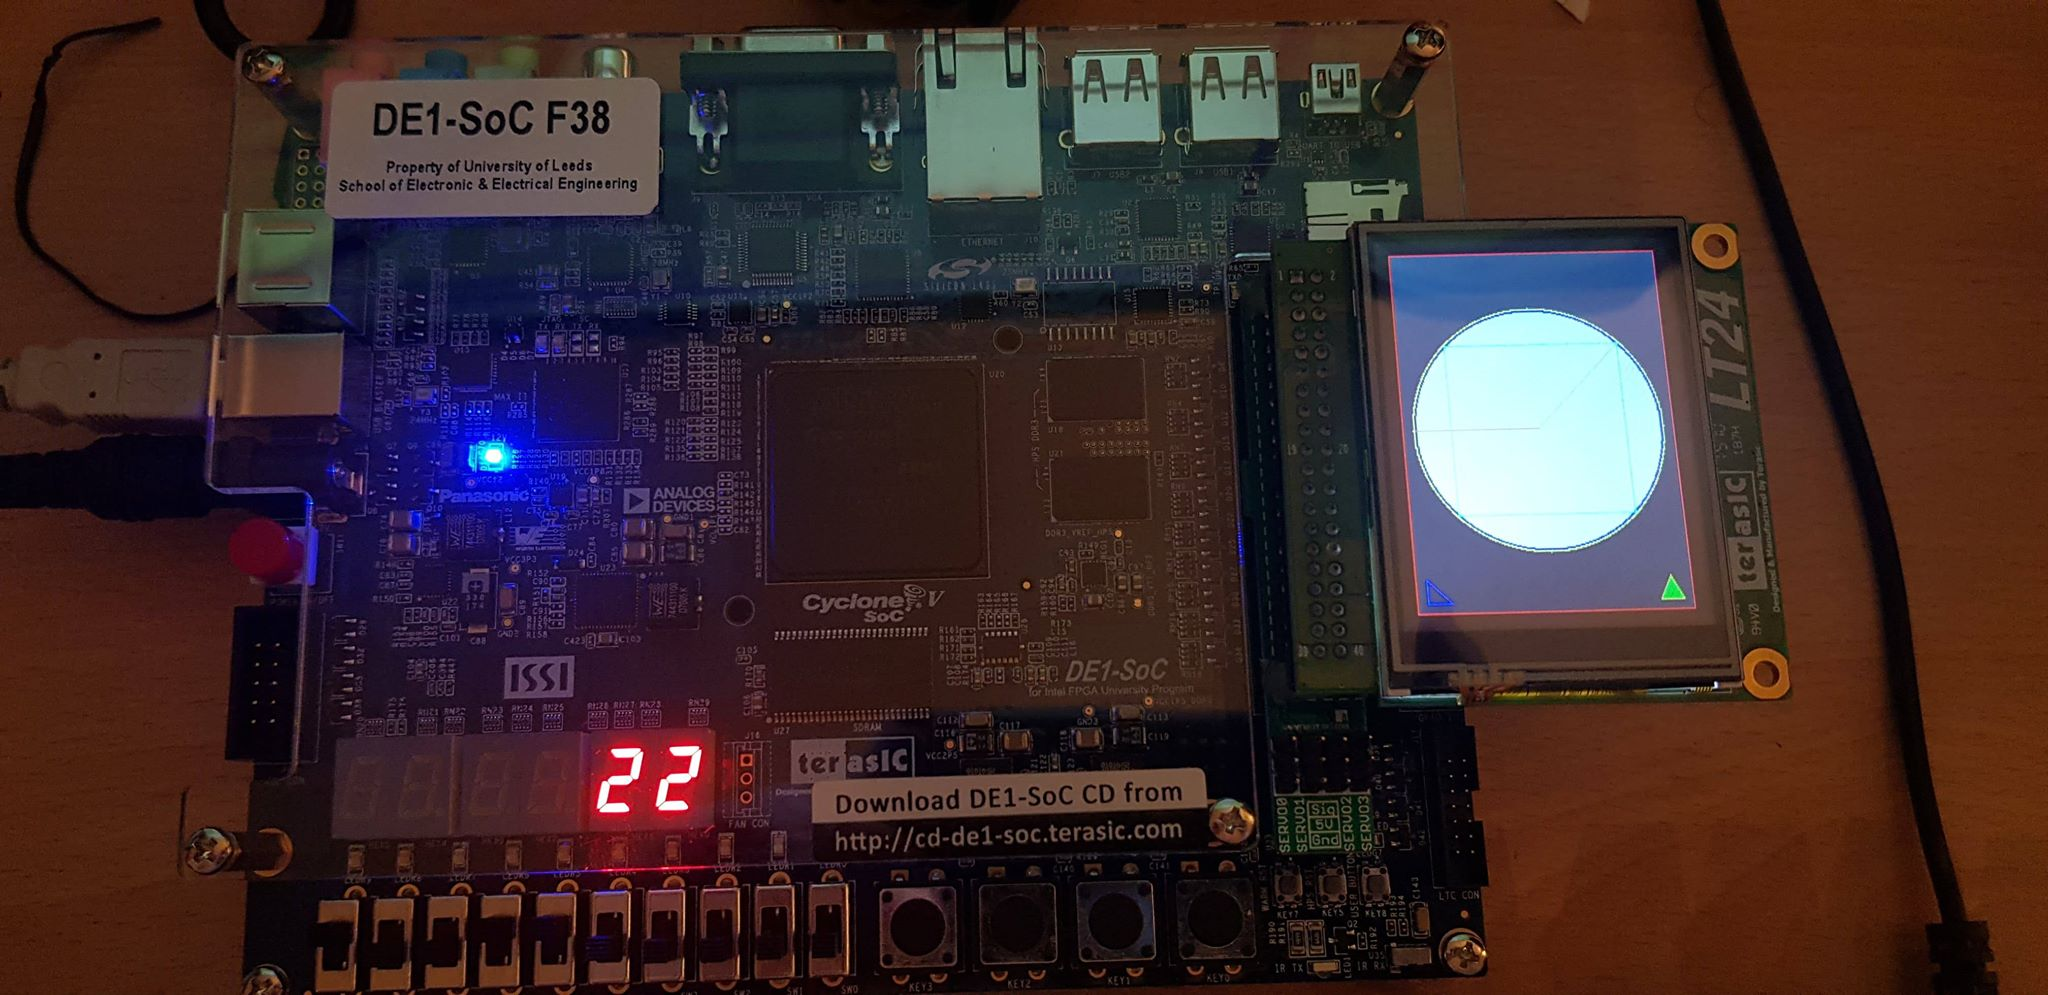
\includegraphics[width=0.5\textwidth]{WorkingPic.jpg}}
	\caption{The final working driver displayed on the DE1-SoC}
\end{figure}

\begin{flushleft}
In this assignment there was 3 different prerequisite's, firstly build a simple driver with a source file and a header file, secondly it must be able to draw lines, circles, rectangles, and triangles, finally the shapes must also allow the option to be filled and unfilled. [1] A piece of test code was provided to which produces a test image. This can be seen in appendix 6.1. 
\newline
\newline
The graphics driver utilised the LT24 display driver. It used the function of LT24 drawPixel and initialisation. The graphics driver comprises of algorithms to create the shapes utilising loops. Every pixel drawn is checked to see if it is still in the window of the LCD screen. A window is a defined area which is within the LCD screen. A wrapper was also created to control the 7 segment display to allow the FPS speed to be outputted onto the board.
\end{flushleft}

\begin{figure}[h]
	\centering
	\fbox{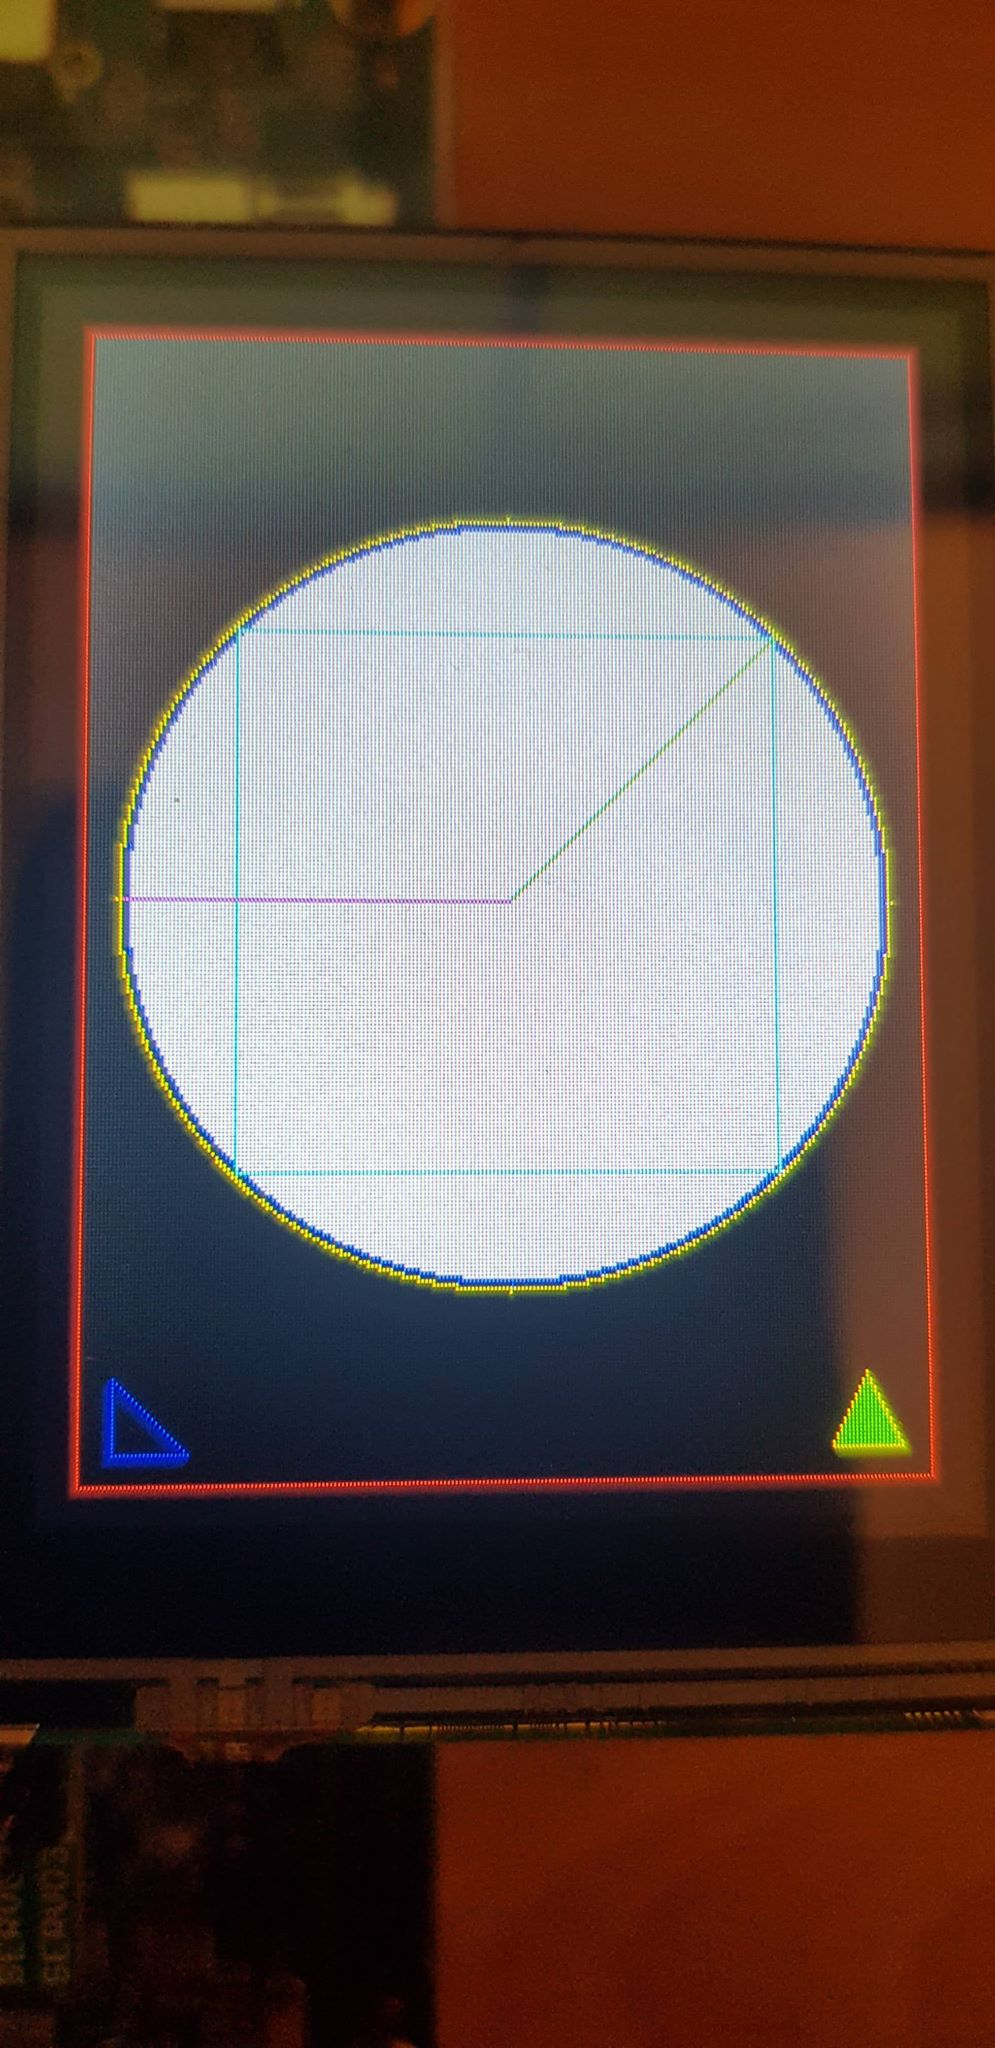
\includegraphics[width=0.2\textwidth]{WCloseUp.jpg}}
	\caption{A close up of the final working driver on the LT24 screen}
\end{figure}
\newpage
\section{Code Design and checking}
\subsection{Draw Pixel}
\begin{figure}[h]
	\centering
	\setlength{\belowcaptionskip}{-15pt}
	\lstinputlisting[language=C++, firstline=204, lastline=212]{\GraphicsC}
	\caption{The function to draw pixel}
\end{figure}
\begin{flushleft}
This function was created to check each pixel is within the LCD window. If a pixel is set outside of the window then the status outputted is not equal to 0. If this happens then the 7 segment display is set to display "E1" for error 1. When error checking is enabled as such in this function it significantly slows down the rendering process for all shapes. An example of this was with hardware optimisation disabled the LCD outputs at 14 FPS. However when enabled it the LCD outputs at 6 FPS. This is a significant reduction in speed. To compensate for this reduction of speed the watchdog would have to be reset as it was causing time outs. Incorporated this to be reset every pixel to prevent a time out.
\end{flushleft}
\subsection{Draw Box}
\begin{flushleft}
The draw box function uses a number of steps to create a box (code in Appendix 6.2.3). Firstly it finds the lowest bottom left corner value of the box by finding the smallest x and smallest y value. It then uses a calculated value for height and width and creates the box using 2 for loops which renders the box one pixel at a time in a typewriter style. Finally, the outline is added to the box.
\end{flushleft}
\subsection{Draw Circle}
\begin{flushleft}
To draw the circle an algorithm was designed utilising Pythagoras theorem (code in Appendix 6.2.4). Pythagoras theorem states that the square of the hypotenuse is equal to the sum of the squares of the other two sides. \newline \newline When used on a grid such as in Figure 5 where you keep R (the hypotenuse) as the radius and cycle through all Y and X co-ordinates it will create a circle. When doing this programmatically you can create an outline by checking if R is equal to the radius and the fill of the shape by checking if it is smaller than R. A threshold had to be used to ensure that the circle has a full outline and not just 12 dots which will appear if only set the equal R. This specific code can be seen on Appendix 6.2.4 lines 12 to 25. 
\newline
\newline
\end{flushleft}
\begin{figure}[h]
	\centering
	\[ x^2 + y^2 = r^2 \]
	\caption{Pythagoras Theorem}
\end{figure}
\begin{figure}[h]
	\centering
	\setlength{\belowcaptionskip}{-15pt}
	\fbox{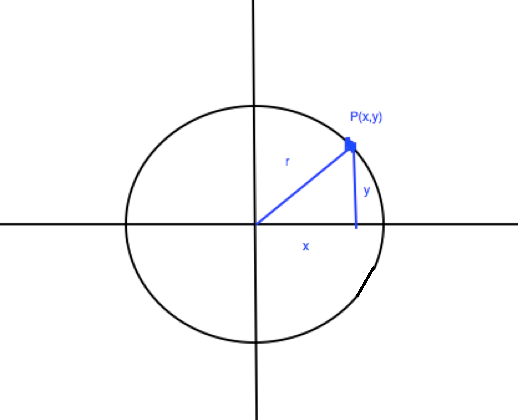
\includegraphics[width=0.5\textwidth]{PythagCircle.png}}
	\caption{Pythagoras theorem to create circle diagram [n]}
\end{figure}

\subsection{Draw Line}
\begin{flushleft}
To draw the line (code in appendix 6.2.5) it was more difficult than expected. An algorithm called Bresenham's line algorithm. The code was based off an example found on Rosetta code. [3]  The algorithm essentially draws a line across the pixels. If error 2 is larger than dy then x1 is equal to x1 plus a value dependent on the quadrant which the line's angle lies in. If error 2 is smaller than dx then error is increased by dx and y1 is equal to y1 plus a value dependent on the quadrant. This can be better shown in figure 6 where sx and sy are set depending on the quadrant. This turns on the appropriate pixels of where the line lands.
\end{flushleft}
\begin{figure}[h]
	\centering
	\setlength{\belowcaptionskip}{-15pt}
	\lstinputlisting[language=C++, firstline=134, lastline=148]{\GraphicsC}
	\caption{The function to draw pixel}
\end{figure}
\subsection{Draw Triangle}
\begin{flushleft}
To draw a triangle two functions where created. One function created the outline using the line function and another function was created which was a modification of the line function to fill the triangle. \newline \newline
This modified version of the line function created worked by creating numerous straight lines from with one point set to x3,y3, and another set which moves between x1,y1 and x1,y2. This code was run 3 times to ensure it is filled as in smaller triangles the lines are more distorted. This modification was a single line of code on line 2 of Figure 8.
\end{flushleft}
\begin{figure}[h]
	\centering
	\setlength{\belowcaptionskip}{-15pt}
	\lstinputlisting[language=C++, firstline=151, lastline=164]{\GraphicsC}
	\caption{The main triangle function}
\end{figure}
\begin{figure}[h]
	\centering
	\setlength{\belowcaptionskip}{-15pt}
	\lstinputlisting[language=C++, firstline=189, lastline=201]{\GraphicsC}
	\caption{The fill triangle function sample showing the single line modification}
\end{figure}
\begin{flushleft}
.
\newline
\newline
\end{flushleft}
\section{Testing and Debugging}
\begin{flushleft}
Various testing techniques were used to test both software and hardware using the graphics driver.
\end{flushleft}
\subsection{Software}
In software testing and debugging the Eclipse IDE was used to step through code and test variables to see if they are to be as what is expected. A number of bugs were solved by doing this, an example was such as when a boolean NOT symbol was used instead of the logical NOT symbol (!) which stopped fills working correctly for the shapes as this made the if statements act erratically. \newline \newline Another example of using this method was testing the timer where it was possible to grab the variables to find how long it took the DE1-SoC to run the test code. A breakpoint would be placed on line 6 of Figure 9 allowing the variables to be seen in the variable explorer in the debugger. Using this for the timer the hardware optimisation code was tested which was enabled from the LT24 driver. It was found that when the hardware optimisation was enabled that the frame rate decreased from 6 FPS to 3 FPS.
\begin{figure}[h]
	\centering
	\setlength{\belowcaptionskip}{-15pt}
	\lstinputlisting[language=C++, firstline=32, lastline=37]{\TimerC}
	\caption{The timer stop function snippet}
\end{figure}

\subsection{Hardware}
When testing on hardware the example code would be run and checked to see if it was as displayed as expected. The frame rate was outputted from the timer to the 7 segment display using a library which was created. (Appendix 6.4) The error function was also tested by trying to draw a pixel which was not on the physical screen which displayed error E1 on the 7 segment display.
\section{Conclusion}
\begin{flushleft}
In conclusion, creating the Graphics driver was an intellectually stimulating task in which numerous algorithms and testing techniques had to be used. The most difficult challenges were the create a line algorithm and triangle fill algorithm. The Eclipse IDE was found to be a very powerful tool for testing and debugging as it allows us to step through code whilst checking registers and memory variables. The final graphics driver was a success however did not run as fast as wanted. More optimisation would've been possible with more time which could have increased the frames per second. 
\end{flushleft}
\newpage
\section{Appendix}
\subsection{Test code}
\lstinputlisting[language=C++]{testcode.cpp}
\subsection{Graphics.c/.h}
\subsubsection{Graphics Header}
\lstinputlisting[language=C++]{\GraphicsH}
\subsubsection{Graphics initialise}
\lstinputlisting[language=C++, firstline=2, lastline=4]{\GraphicsC}
\newpage
\subsubsection{Graphics drawBox}
\lstinputlisting[language=C++, firstline=6, lastline=64]{\GraphicsC}
\subsubsection{Graphics drawCircle}
\lstinputlisting[language=C++, firstline=66, lastline=106]{\GraphicsC}
\newpage
\subsubsection{Graphics drawLine}
\lstinputlisting[language=C++, firstline=108, lastline=149]{\GraphicsC}
\newpage
\subsubsection{Graphics drawTriangle}
\lstinputlisting[language=C++, firstline=151, lastline=164]{\GraphicsC}
\newpage
\subsubsection{Graphics fillTriangle}
\lstinputlisting[language=C++, firstline=166, lastline=202]{\GraphicsC}
\subsubsection{Graphics drawPixel}
\lstinputlisting[language=C++, firstline=204, lastline=212]{\GraphicsC}

\newpage
\subsection{Timer.c/.h}
\subsubsection{Timer Header}
\lstinputlisting[language=C++]{\TimerH}
\subsubsection{Timer start}
\lstinputlisting[language=C++, firstline=14, lastline=26]{\TimerC}
\subsubsection{Timer stop}
\lstinputlisting[language=C++, firstline=28, lastline=41]{\TimerC}

\newpage
\subsection{sevenSeg.c/.h}
\subsubsection{SDisplay Header}
\lstinputlisting[language=C++]{\sevenSegH}
\subsubsection{SDisplay clearAll}
\lstinputlisting[language=C++, firstline=24, lastline=32]{\sevenSegC}
\subsubsection{SDisplay set}
\lstinputlisting[language=C++, firstline=5, lastline=22]{\sevenSegC}
\newpage

\section{Bibliography}
[1] D. Cowell, S. Freear and T. Carpenter, "ELEC5620M: Embedded Microprocessor System Design - Assignment 1", 2019. \newline
[2] Veritas Prep, Pythagoras Theorem to create circle. 2016 [Online]. Available: \newline https://www.veritasprep.com/blog/wp-content/uploads/2016/10/DG-Blog-4.png. [Accessed: 19-Mar-2019]. \newline
[3]"Bitmap/Bresenham's line algorithm - Rosetta Code", Rosettacode.org. [Online]. Available: https://rosettacode.org/wiki/Bitmap/Bresenham\%27s\_line\_algorithm. [Accessed: 19-Mar-2019] \newline
\end{document}